	En este capítulo comparamos los resultados de la ejecución de 5 modelos, los tiempos de ejecución de cada modelo en PowerDEVS comparándolos con 
	el modelo transformado en QSS-Solver. 
	Los modelos ejecutados tanto los originales, en PowerDEVS, y los modelos 
	transformados en $\mu$-Modelilca se encuentran en \url{https://github.com/lucciano/pd2mo/tree/master/doc/tesina/src}

\section{Comparación de performance}
	A continuación por cada uno de los modelos se muestra su modelo en PowerDEVS seguido de dos gráficas (ambas son generadas con GNUPlot), 
	a la izquierda se muestra el resultado de la simulación de PowerDEVS y a la derecha el resultado del modelo transformado en el QSS-Solver.

	Las simulaciones fueron llevadas acabo en una PC Intel\textsuperscript{\textregistered} Core\textsuperscript{TM} i7-3632QM CPU @ 2.20GHz con 16 GB de memoria RAM. Los tiempos observados no deben ser considerados como absolutos ya que variarán de un sistema a otro, aun que las mejoras relativas se mantendrán.


\section{Ecuaciones Lotka-Volterra}

	El sistema de ecuaciones Lotka-Volterra fue presentado en la página \pageref{lotka_volterra_ref}, es un sistema de ecuaciones diferenciales de primer orden, no lineales, utilizadas para describir dinámicas de sistemas biológicos en el cual dos especies interactúan, una como presa y otra como depredador, se definen como:

\begin{align*}
\frac{dx}{dt} & = x(\alpha - \beta y)\\
\frac{dy}{dt} & =y(\gamma - \delta  x)
\end{align*}

donde:
\begin{itemize}
	\item y es el número de algún predador (por ejemplo, un lobo);
    \item x es el número de sus presas (por ejemplo, conejos);
    \item t representa el tiempo; y
    \item $\alpha$, $\beta$, $\gamma$, $\delta$ son parámetros que representan las interacciones de las dos especies.
\end{itemize}

	Este sistema es representado en PowerDEVS por el modelo de la figura \ref{lotka_voltera_pwd}:

\begin{figure}[H]
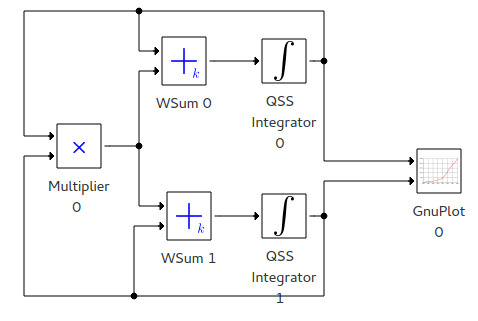
\includegraphics[width=0.75\linewidth]{lotka_voltera_pwd}
\caption{Modelo PowerDEVS del Sistema Lotka Volterra}
\label{model:lotka_voltera}
\end{figure}

\begin{figure}[H]
\centering
\begin{minipage}{0.5\textwidth}
\centering
 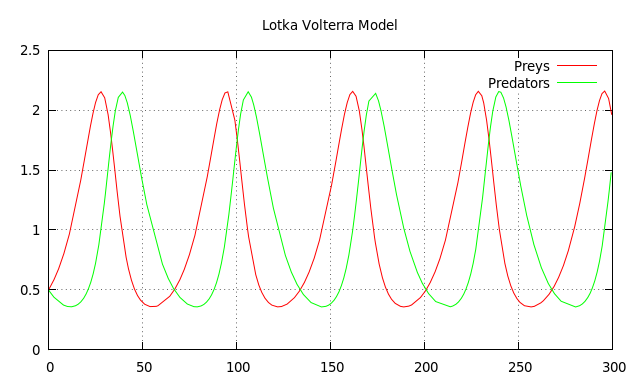
\includegraphics[width=\linewidth]{lotka_voltera-pd}
PowerDEVS \\
\end{minipage}\hfill
\begin{minipage}{0.5\textwidth}
\centering
 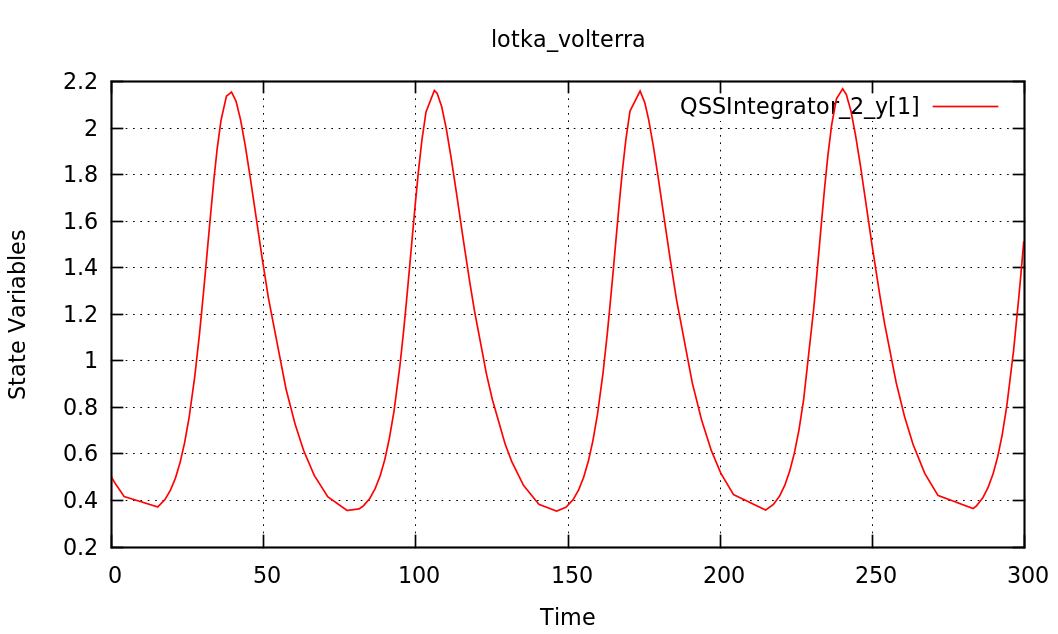
\includegraphics[width=\linewidth]{lotka_voltera-qss}
QSS-Solver \\
\end{minipage}
\label{graph:lotka_voltera}
\caption{Resultados de la simulación del Modelo Lotka Volterra}
\end{figure}

En la figura \ref{graph:lotka_voltera} se pueden ver los dos resultados de la simulación de 300 segundos a la izquierda el resultado en PowerDEVS, el cual tomo 11ms,
y a la derecha el resultado en QSS-Solver el cual tomo 2.75ms.

\section{Líneas de Transmisión}
	El siguiente sistema de ecuaciones representan un modelo de una línea de transmisión formada por $N$ secciones de circuitos LC:

\begin{equation}
\begin{split}
\frac{d v_{j}}{d t} &= \frac{i_{j} - i_{j+1}}{C} \\
\frac{d i_{j}}{d t} &= \frac{v_{j-1} - v_{j}}{L} \\	
\end{split}
\end{equation}

para $j = 2 \dots N$

Consideramos un pulso de entrada:
\begin{equation}
v_0(t) = \left\{ 
  \begin{array}{l l}
    1 \text{ si } t < 1 \\
    0 \text{ en caso contrario }
  \end{array} \right.
\end{equation}

En la figura \ref{model:lclines} se puede ver el modelo de PowerDEVS para la simulación del modelo de Líneas de Transmisión.

\begin{figure}[H]
 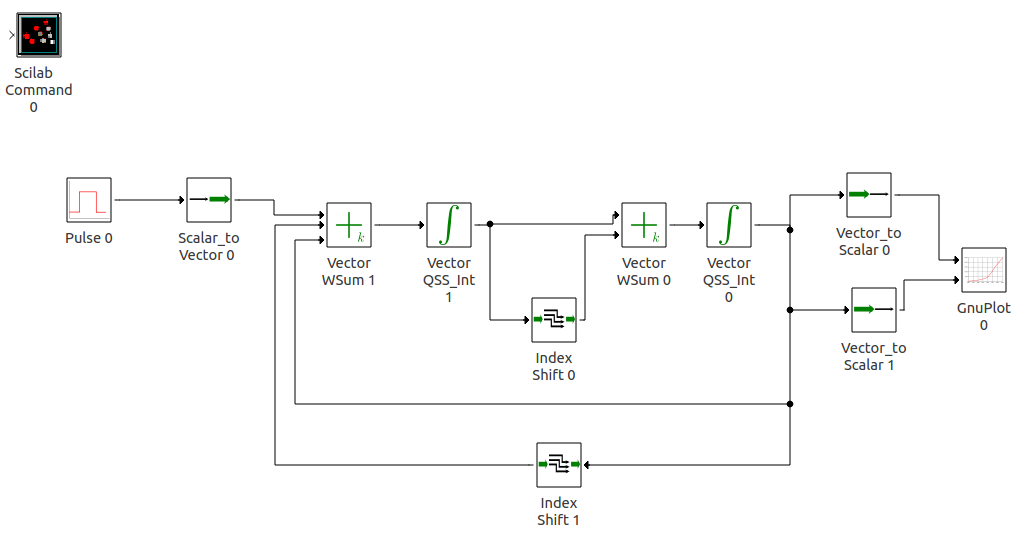
\includegraphics[width=0.75\linewidth]{lclines}
\label{model:lclines}
\caption{Modelo PowerDEVS de Líneas de Transmisión}
\end{figure}

\begin{figure}[H]
\centering
\begin{minipage}{0.5\textwidth}
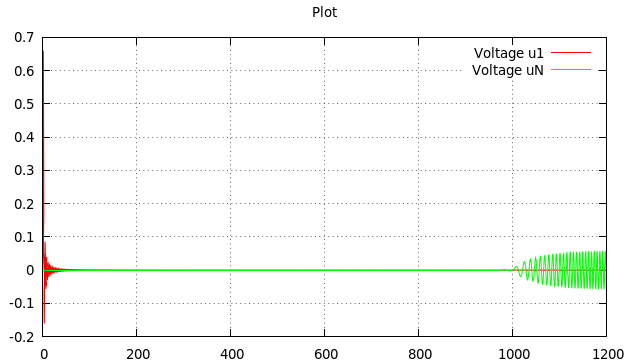
\includegraphics[width=\linewidth]{lcline-pd}
PowerDEVS\\
\end{minipage}\hfill
\begin{minipage}{0.5\textwidth}
 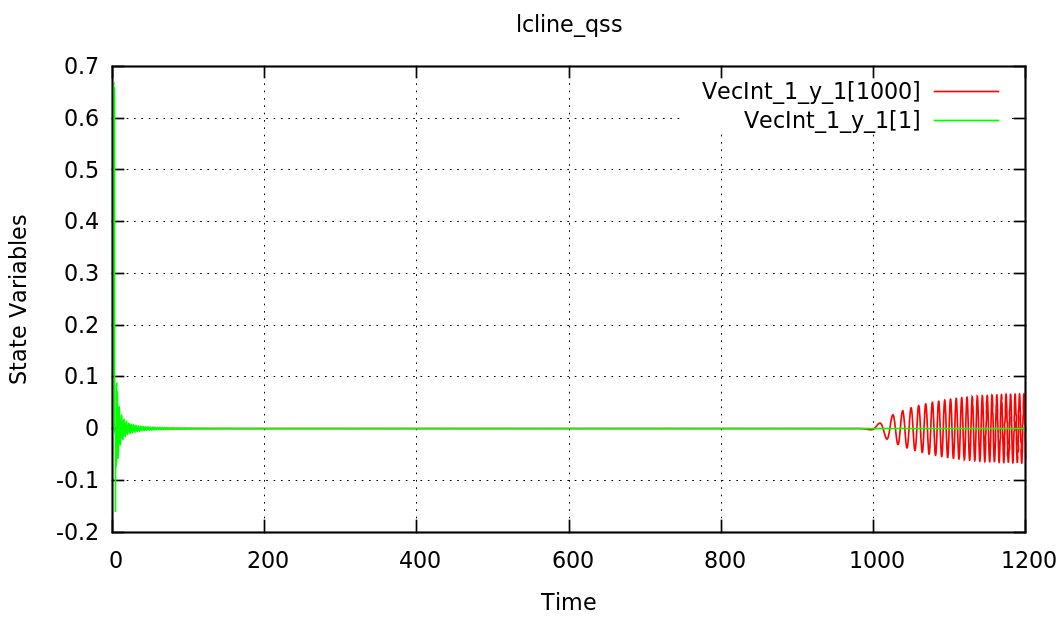
\includegraphics[width=\linewidth]{lcline-qss}
QSS-Solver\\
\end{minipage}
\caption{Resultados de la simulación de Líneas de Transmisión}
\label{graph:lclines}
\end{figure}

En la figure \ref{graph:lclines} se puede ver el resultado de la simulación de 20 minutos (1200s) del Modelo de Líneas de Transmisión con 1000 segmentos en PowerDEVS,
	la cual tomo 76402ms a la izquierda, mientras que a la derecha se encuentra el resultado del modelo convertido ejecutado en con los mismo parámetros en
	QSS-Solver, el cual tomo 34982.5ms.

\section{Inversores Lógicos}
	El siguiente modelo representa una cadena de $m$ inversores lógicos, 

\begin{align*}
\frac{d \omega_1}{d t} & = U_{op} - \omega_1(t) - \Upsilon g (u_{in}(t), \omega_{1} (t))    \\
\frac{d \omega_j}{d t} & = U_{op} - \omega_j(t) - \Upsilon g (\omega_{j-1}(t), \omega_{j} (t)) \textrm{ donde $j = 2, 3, .., m$}
\end{align*}


\begin{figure}[H]
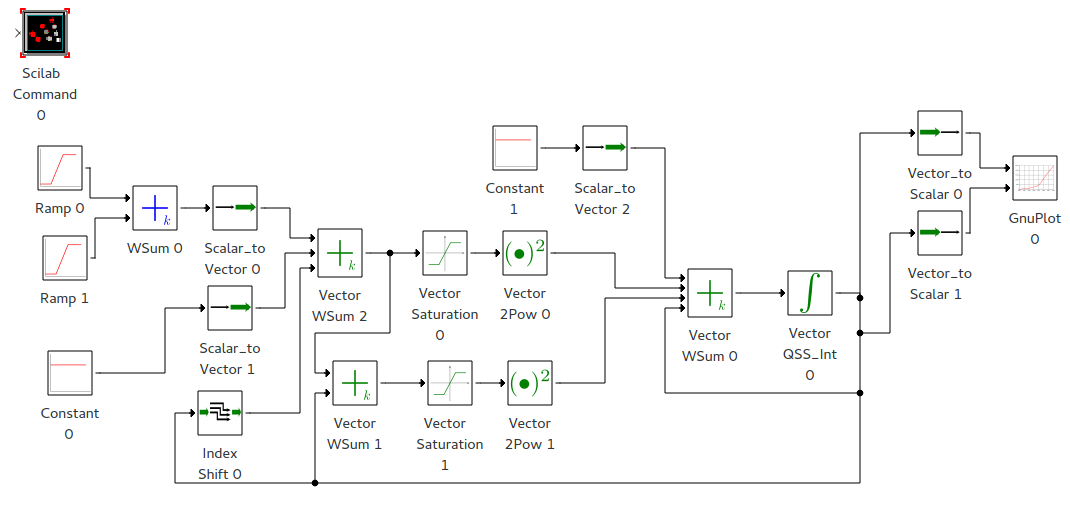
\includegraphics[width=0.75\linewidth]{inverters}
\label{model:inverters}
\caption{Modelo PowerDEVS de Inversores Lógicos}
\end{figure}

\begin{figure}[H]
\centering
\begin{minipage}{0.5\textwidth}
 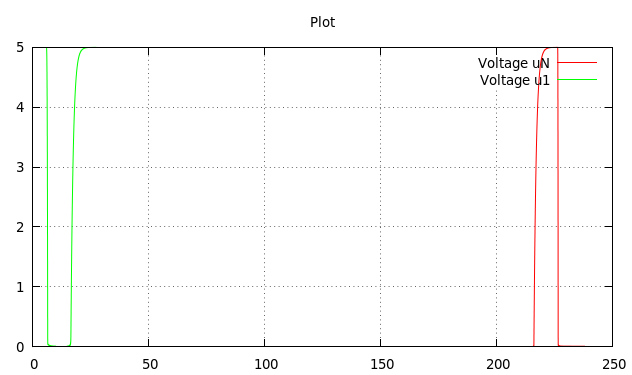
\includegraphics[width=\linewidth]{inversers-pd}
\centering
PowerDEVS
\end{minipage}\hfill
\begin{minipage}{0.5\textwidth}
 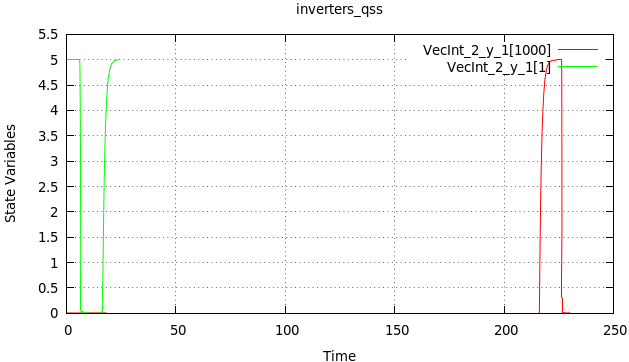
\includegraphics[width=\linewidth]{inversers-qss}
\centering
QSS-Solver
\end{minipage}
\caption{Resultados de la simulación de Inversores}
\label{graph:inverters}
\end{figure}

En la figura \ref{graph:inverters} se puede ver el resultado de la simulación del modelo de 1000 inversores durante 250 segundos, lo cual tomo 25046ms en PowerDEVS en 
	la izquierda, mientras que en QSS-Solver tomo 7694.44ms	

\section{Advection-Diffusion-Reaction}
	El modelo de ecuaciones Advection-diffusion-reaction (ADR) provee las bases para describir fenómenos de transferencias de calor y masa, donde la cantidad de interés $u(x,t)$ puede ser temperatura en la conducción de calor o concentración de una sustancia química.

La ecuación 
\begin{equation*}
\frac{du(x,t)}{dt} + a \frac{du(x,t)}{dx} = d\frac{d^2u(x,t)}{d^2x} + r(u(x,t)^2 - u(x,t)^3)
\end{equation*}
corresponde al modelo ADR, donde $a$,$d$ y $r$ son parámetros expresando coeficientes de advección, difusión y reacción

\begin{figure}[H]
 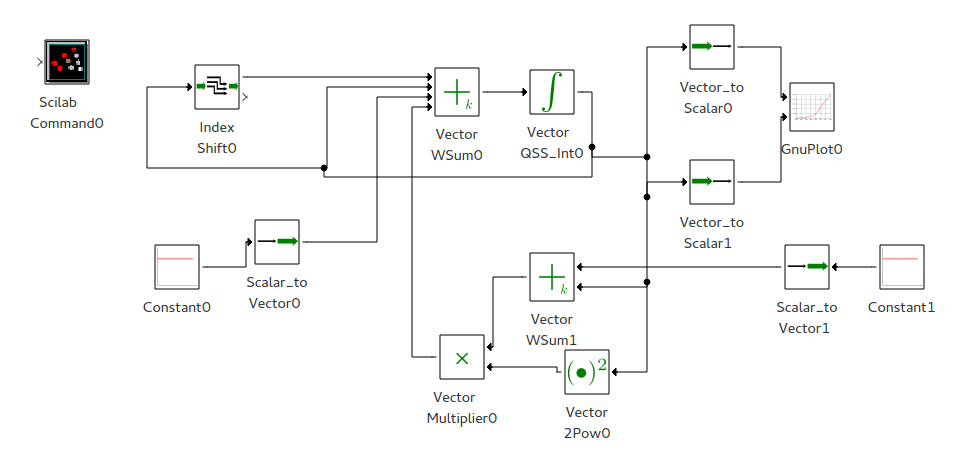
\includegraphics[width=0.75\linewidth]{adr-pwd}
\label{model:adr}
\caption{Modelo PowerDEVS ADR}
\end{figure}

\begin{figure}[H]
\begin{minipage}{0.5\textwidth}
 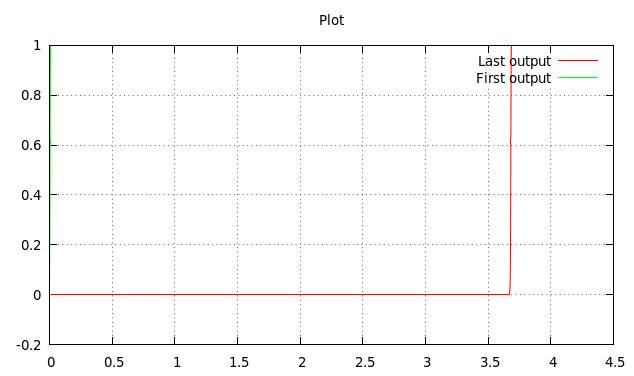
\includegraphics[width=\linewidth]{adr-pd}
\centering
PowerDEVS
\end{minipage}\hfill
\begin{minipage}{0.5\textwidth}
 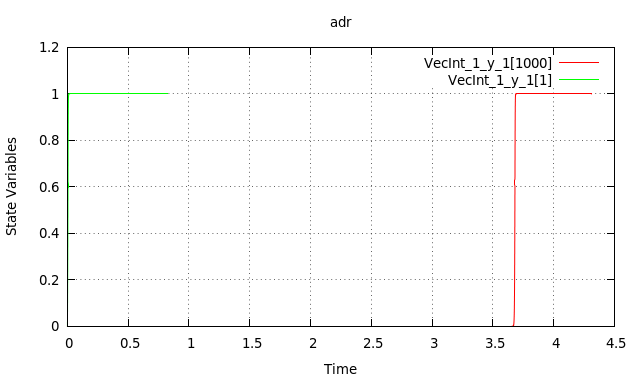
\includegraphics[width=\linewidth]{adr-qss}
\centering
QSS-Solver
\end{minipage}
\label{graph:adr}
\caption{Resultados de la simulación ADR}
\end{figure}

En la figura \ref{graph:adr} se puede ver el resultado de la simulación del modelo ADR de 10s para $N=1000$ en PowerDEVS a la izquierda, la cual tomo 6089ms,
mientras que la simulación QSS-Solver del modelo convertido es 568.772ms, en ambos casos utilizando el método de integración LIQSS2.

\section{Convertidor de Voltaje}
	El siguiente modelo es un tipo de convertidor DC - DC que obtiene a su  salida  un  voltaje  continuo  menor  que  a  su entrada, manteniendo una una  alta eficiencia (superior al 95\% con circuitos integrados) y autorregulación.

\begin{align*}
\frac{di_{L}}{dt} & = \frac{-u_{C} - R_D i_D }{L}\\
\frac{du_C}{dt} & =i_D \frac{i_D}{C} - \frac{u_C}{R_L C }
\end{align*}
donde
\begin{align*}
i_D & = \frac{R_s i_L - u_C - U }{R_D + R_s}
\end{align*}


\begin{figure}[H]
\centering
 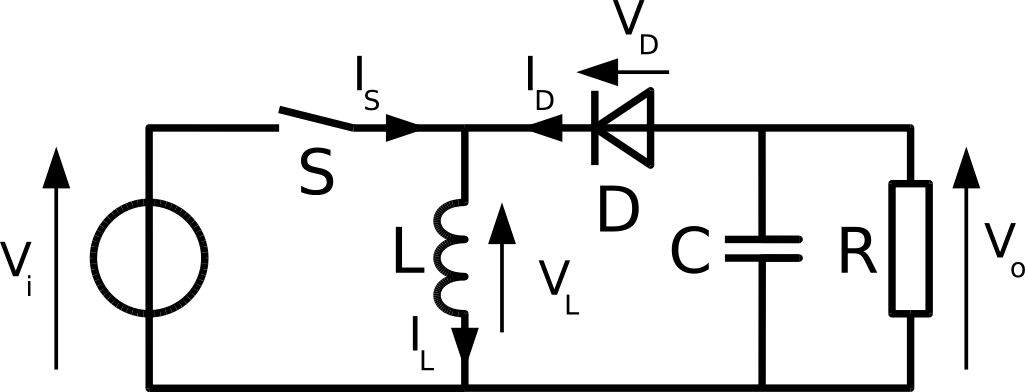
\includegraphics[width=.60\linewidth]{Buckboost_conventions}
 \label{buckdisk-squema}
 \caption{Esquema eléctrico de convertidor de voltaje en PowerDEVS}
\end{figure}

\begin{figure}[H]
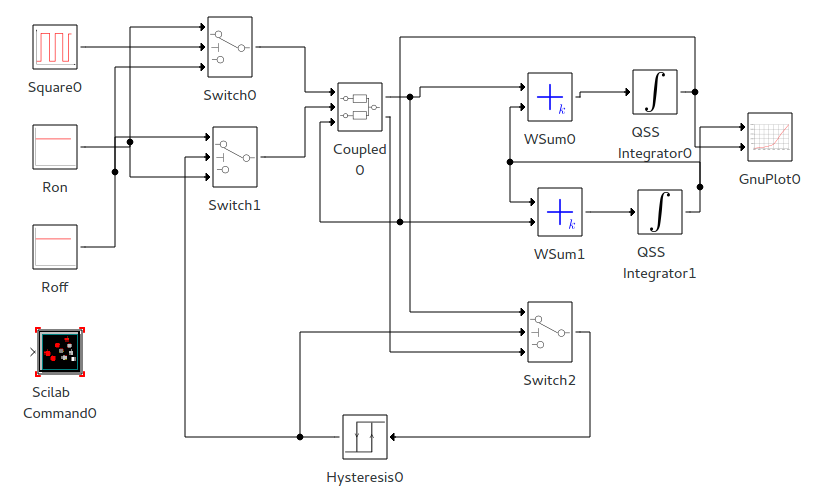
\includegraphics[width=0.75\linewidth]{buck_disk}
 \label{model:buckdisk}
\caption{Modelo Convertidor de voltaje}
\end{figure}

\begin{figure}[H]
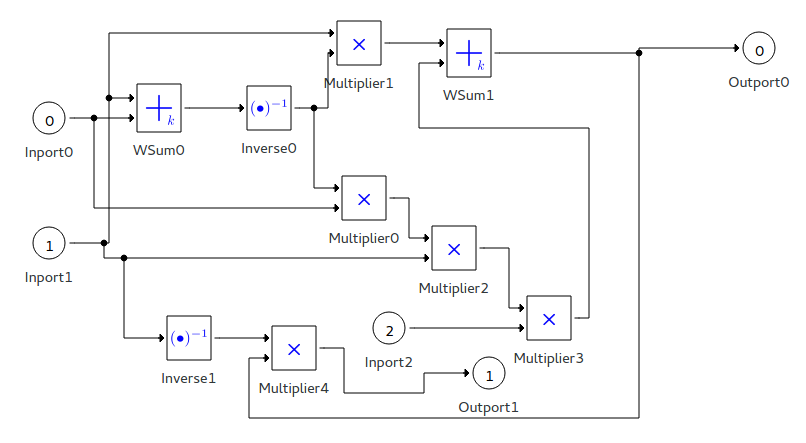
\includegraphics[width=0.75\linewidth]{buck_disk_coupled0}
\caption{Coupled0 (Incluido en Convertidor de voltaje)}
\label{model:buckdisk_coupled0}
\end{figure}

\begin{figure}[H]
\begin{minipage}{0.5\textwidth}
 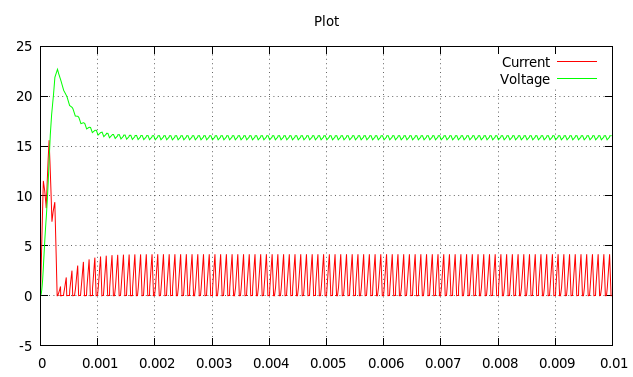
\includegraphics[width=\linewidth]{buck_disk-pd}
\centering
PowerDEVS
\label{model:buckdisk_coupled0}
\end{minipage}\hfill
\begin{minipage}{0.5\textwidth}
 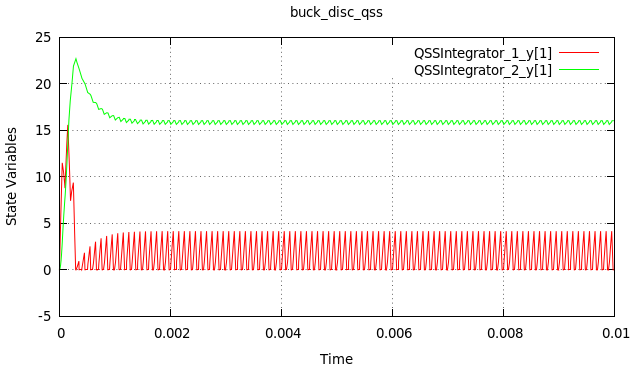
\includegraphics[width=\linewidth]{buck_disk-qss}
\centering
QSS-Solver
\label{model:buckdisk}
\end{minipage}
\caption{Resultados de la simulación de Convertidor de voltaje}
\end{figure}

En la figura \ref{model:buckdisk} se puede ver el resultado del modelo de Convertidor de voltaje durante 0.01s a la izquierda en PowerDEVS, lo cual tomo 268ms, 
mientras que a la derecha se encuentra el resultado obtenido del QSS-Solver, el cual tomo 10ms.

\section{Resultados}

	Cada una de las simulaciones fue realizadas en una PC Intel\textsuperscript{\textregistered} Core\textsuperscript{TM} i7-3632QM CPU @ 2.20GHz con 16 GB de
	 memoria RAM. Los tiempos observados no deben ser considerados como absolutos ya que variarán de un sistema a otro, pero las mejoras relativas en los tiempos de ejecución deberían mantenerse.

	En el cuadro \ref{tab:result} se sumarizan los tiempos de ejecución obtenidos de los 5 modelos descriptos en este capitulo en  
	PowerDEVS (P.DEVS) y QSS-Solver (QSS-S), ambas mediciones son reportadas por los motores de simulación, en milisegundos (ms),
	 todas las simulaciones utilizan el método de integración QSS3 excepto los que se especifica LIQSS2.

\begin{table}[H]
\centering	
\begin{tabular}{llllll}
\toprule
{\bf Modelos}            &  {\bf P.DEVS(ms)} & {\bf QSS-S. (ms)} & {\bf Mejora (\%)} \\
\toprule
Lotka  Voltera 300s      		& 11            & 2.75132         & 81 \\
Lineas de Transmisión 1200s, N=1000     & 76402         & 34982.5         & 54          \\
Inversores(LIQSS2) 250s, N=1000   	& 25046         & 7694.44         & 69        \\
ADR(LIQSS2) 10s, N=1000 		& 6089          & 568.772         & 90        \\
Convertidor de Voltaje 0.01s,        	& 268           & 10.3802         & 96         

% Mejora esta calculada a partir de 1 - qsssolver / pwdevs
%excepto indicado, se utiliza QSS3
\end{tabular}
\caption{Comparación de las diferentes simulaciones y sus mejoras}\label{tab:result}
\end{table}

	En el cuadro \ref{tab:result} se puede ver una mejora entre 54 y 96\% entre todos los modelos, y entre 54 y 90\% para los modelos vectoriales que son nuestro 
	principal objetivo, ya que son la forma más simple de describir grandes modelos, lo cual es lo esperado al cambiar de formalismo se evita todo los 
	mensajes entre modelos característico del formalismo DEVS.
